% Root file used ashow macros
\documentclass{beamer}
\usepackage{tikz}
\usetikzlibrary{calc,arrows.meta}
\usepackage{xcolor}
\usepackage{multicol}
\usepackage{amsmath}

% ================================================================
% Answer-overlay helpers
% ================================================================
\newcommand{\ablank}[1]{%
  \alt<2>{\textcolor{red}{\underline{#1}}}{\underline{\phantom{#1}}}%
}
\newcommand{\ashow}[1]{\uncover<2->{\textcolor{red}{\small #1}}}
\newcommand{\ashowq}[1]{\alt<2->{\textcolor{red}{\small #1}}{?}}

\title{Areas, Perimeters \& Averages: Worked Solutions}
\author{}
\date{}

\begin{document}

\frame{\titlepage}

%------------------------------------------------
% Contents
%------------------------------------------------
\begin{frame}{Contents}
\small
\begin{itemize}
  \item \textbf{Starter 1: Shapes A, B and C}
  \begin{itemize}
    \item \hyperlink{starter1qs}{Questions and Short Answers}
    \item \hyperlink{starter1work}{First Worked Solution}
  \end{itemize}
  \item \textbf{Starter 2: Shapes D, E and F}
  \begin{itemize}
    \item \hyperlink{starter2qs}{Questions and Short Answers}
    \item \hyperlink{starter2work}{First Worked Solution}
  \end{itemize}
\end{itemize}
\end{frame}

%------------------------------------------------
% Copy of original Slide 1
%------------------------------------------------
\begin{frame}[label=starter1qs]{Starter 1: Questions and Short Answers}

\vspace{-1em}

\begin{columns}

\column{0.38\textwidth}
\begin{center}
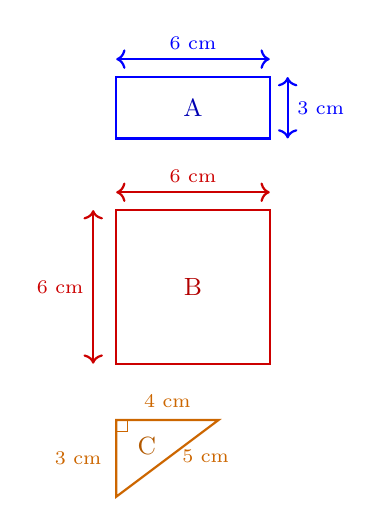
\begin{tikzpicture}[scale=0.65]

  %--- Shape A: Rectangle, 6 cm × 3 cm ---
  \draw[thick, blue] (0,9.5) rectangle (3,8.3);
  \draw[blue, thick, <->] (0,9.85) -- (3,9.85);
  \node[blue, above] at (1.5,9.85) {\scriptsize 6 cm};
  \draw[blue, thick, <->] (3.35,8.3) -- (3.35,9.5);
  \node[blue, right] at (3.35,8.9) {\scriptsize 3 cm};
  \node[blue!70!black] at (1.5,8.9) {\small A};

  %--- Shape B: Square, 6 cm × 6 cm ---
  \draw[thick, red!80!black] (0,6.9) rectangle (3,3.9);
  \draw[red!80!black, thick, <->] (0,7.25) -- (3,7.25);
  \node[red!80!black, above] at (1.5,7.25) {\scriptsize 6 cm};
  \draw[red!80!black, thick, <->] (-0.45,3.9) -- (-0.45,6.9);
  \node[red!80!black, left] at (-0.45,5.4) {\scriptsize 6 cm};
  \node[red!70!black] at (1.5,5.4) {\small B};

  %--- Shape C: Right-angled triangle, legs 4 cm and 3 cm, hypotenuse 5 cm ---
  \draw[thick, orange!80!black] (0,2.8) -- (2,2.8) -- (0,1.3) -- cycle;
  \draw[orange!80!black] (0.22,2.8) -- (0.22,2.58) -- (0,2.58);
  \node[orange!80!black, above] at (1.0,2.85) {\scriptsize 4 cm};
  \node[orange!80!black, left] at (-0.1,2.05) {\scriptsize 3 cm};
  \node[orange!80!black, right] at (1.1,2.1) {\scriptsize 5 cm};
  \node[orange!70!black] at (0.6,2.3) {\small C};

\end{tikzpicture}
\end{center}

\column{0.62\textwidth}
\small
\begin{enumerate}
  \begin{multicols}{2}
    \item $6 \times 3 =$ \ashowq{$18$}
    \item $\frac{3}{24} + \frac{5}{24} =$ \ashowq{$\frac{1}{3}$}
  \end{multicols}
  \begin{multicols}{2}
    \item $\tfrac{1}{2} \times 4 \times 3 =$ \ashowq{$6$}
    \item $-3 \times -2 =$ \ashowq{$6$}
  \end{multicols}
  \item Find the mean of $\ 8,\ 14,\ 20$. \ashow{$14$}
  \item What fraction of $60$ is $6$?\quad Simplify fully. \ashow{$\frac{1}{10}$}
\end{enumerate}

\vspace{-1.2em}

\begin{enumerate}
  \setcounter{enumi}{6}
  \item Find the \textbf{area} of each shape A, B and C. \ablank{$A=18$},\ \ablank{$B=36$},\ \ablank{$C=6$}.
  \item Find the \textbf{perimeter} of each shape A, B and C. \ablank{$A=18$},\ \ablank{$B=24$},\ \ablank{$C=12$}.
  \item Find the \textbf{mean area} of the three shapes. \ablank{$20$}.
  \item Find the \textbf{mean perimeter} of the three shapes. \ablank{$18$}.
  \item What fraction of the total area does shape C make up? \ablank{$\frac{6}{60}=\frac{1}{10}$}.
\end{enumerate}

\end{columns}
\end{frame}

%------------------------------------------------
% Copy of original Slide 2
%------------------------------------------------
\begin{frame}[label=starter2qs]{Starter 2: Questions and Short Answers}

\vspace{-1em}

\begin{columns}

\column{0.38\textwidth}
\begin{center}
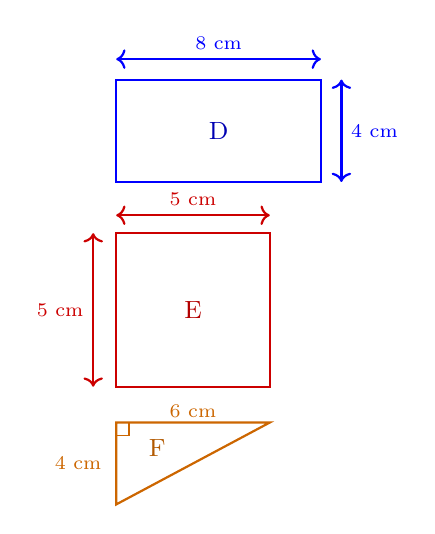
\begin{tikzpicture}[scale=0.65]

  %--- Shape D: Rectangle, 8 cm × 4 cm ---
  \draw[thick, blue] (0,9.5) rectangle (4,7.5);
  \draw[blue, thick, <->] (0,9.9) -- (4,9.9);
  \node[blue, above] at (2,9.9) {\scriptsize 8 cm};
  \draw[blue, thick, <->] (4.4,7.5) -- (4.4,9.5);
  \node[blue, right] at (4.4,8.5) {\scriptsize 4 cm};
  \node[blue!70!black] at (2,8.5) {\small D};

  %--- Shape E: Square, 5 cm × 5 cm ---
  \draw[thick, red!80!black] (0,6.5) rectangle (3,3.5);
  \draw[red!80!black, thick, <->] (0,6.85) -- (3,6.85);
  \node[red!80!black, above] at (1.5,6.85) {\scriptsize 5 cm};
  \draw[red!80!black, thick, <->] (-0.45,3.5) -- (-0.45,6.5);
  \node[red!80!black, left] at (-0.45,5) {\scriptsize 5 cm};
  \node[red!70!black] at (1.5,5) {\small E};

  %--- Shape F: Right-angled triangle, legs 6 cm and 4 cm ---
  \draw[thick, orange!80!black] (0,2.8) -- (3,2.8) -- (0,1.2) -- cycle;
  \draw[orange!80!black] (0.25,2.8) -- (0.25,2.55) -- (0,2.55);
  \node[orange!80!black, above] at (1.5,2.7) {\scriptsize 6 cm};
  \node[orange!80!black, left] at (-0.1,2.0) {\scriptsize 4 cm};
  \node[orange!70!black] at (0.8,2.3) {\small F};

\end{tikzpicture}
\end{center}

\column{0.62\textwidth}
\small
\begin{enumerate}
  \begin{multicols}{2}
    \item $8 \times 4 =$ \ashowq{$32$}
    \item $\frac{7}{20} + \frac{9}{20} =$ \ashowq{$\frac{4}{5}$}
  \end{multicols}
  \begin{multicols}{2}
    \item $\tfrac{1}{2} \times 6 \times 4 =$ \ashowq{$12$}
    \item $-5 \times 4 =$ \ashowq{$-20$}
  \end{multicols}
  \item Find the mean of $\ 6,\ 12,\ 18$. \ashow{$12$}
  \item What fraction of $80$ is $12$?\quad Simplify fully. \ashow{$\frac{3}{20}$}
\end{enumerate}

\vspace{-1.2em}

\begin{enumerate}
  \setcounter{enumi}{6}
  \item Find the \textbf{area} of each shape D, E and F. \ablank{$D=32$},\ \ablank{$E=25$},\ \ablank{$F=12$}.
  \item Find the \textbf{perimeter} of each shape D, E and F. \ablank{$D=24$},\ \ablank{$E=20$},\ \ablank{$F=10+2\sqrt{13}$}.
  \item Find the \textbf{mean area} of the three shapes. \ablank{$23$}.
  \item Find the \textbf{mean perimeter} of the three shapes. \ablank{$\frac{54+2\sqrt{13}}{3}$}.
  \item What fraction of the total area does shape F make up? \ablank{$\frac{12}{69}=\frac{4}{23}$}.
\end{enumerate}

\end{columns}
\end{frame}

%------------------------------------------------
% Worked Solutions: Starter 1
%------------------------------------------------
\begin{frame}[label=starter1work]{Starter 1 -- Q1: Multiplication}
\small
\(6 \times 3\) means 6 groups of 3.

\[
6 \times 3 = 18
\]

Final answer: \(\boxed{18}\).
\end{frame}

\begin{frame}{Starter 1 -- Q2: Adding Fractions}
\small
The denominators are already the same, so add the numerators:

\[
\frac{3}{24}+\frac{5}{24}
=\frac{3+5}{24}
=\frac{8}{24}
\]

Simplify by dividing the numerator and denominator by 8:

\[
\frac{8}{24}=\frac{1}{3}
\]

Final answer: \(\boxed{\frac{1}{3}}\).
\end{frame}

\begin{frame}{Starter 1 -- Q3: Triangle Area}
\small
Use the triangle area formula:

\[
A=\frac12 \times \text{base} \times \text{height}
\]

Here the base is 4 and the height is 3:

\[
\frac12 \times 4 \times 3 = 2 \times 3 = 6
\]

Final answer: \(\boxed{6}\).
\end{frame}

\begin{frame}{Starter 1 -- Q4: Negative Multiplication}
\small
Multiplying two negative numbers gives a positive product:

\[
-3 \times -2 = 6
\]

Final answer: \(\boxed{6}\).
\end{frame}

\begin{frame}{Starter 1 -- Q5: Mean}
\small
Mean is the sum of the values divided by how many values there are:

\[
\frac{8+14+20}{3}=\frac{42}{3}=14
\]

Final answer: \(\boxed{14}\).
\end{frame}

\begin{frame}{Starter 1 -- Q6: Fraction of 60}
\small
The required fraction is

\[
\frac{6}{60}
\]

Simplify by dividing numerator and denominator by 6:

\[
\frac{6}{60}=\frac{1}{10}
\]

Final answer: \(\boxed{\frac{1}{10}}\).
\end{frame}

\begin{frame}{Starter 1 -- Q7: Areas of A, B and C}
\small
\textbf{Shape A} is a \(6\text{ cm}\times 3\text{ cm}\) rectangle:

\[
A=6\times 3=18\text{ cm}^2
\]

\textbf{Shape B} is a \(6\text{ cm}\times 6\text{ cm}\) square:

\[
B=6\times 6=36\text{ cm}^2
\]

\textbf{Shape C} is a right-angled triangle with legs \(4\text{ cm}\) and \(3\text{ cm}\):

\[
C=\frac12 \times 4 \times 3=6\text{ cm}^2
\]

Final answers: \(\boxed{A=18\text{ cm}^2,\ B=36\text{ cm}^2,\ C=6\text{ cm}^2}\).
\end{frame}

\begin{frame}{Starter 1 -- Q8: Perimeters of A, B and C}
\small
\textbf{Shape A} rectangle:

\[
A=2(6+3)=2\times 9=18\text{ cm}
\]

\textbf{Shape B} square:

\[
B=4\times 6=24\text{ cm}
\]

\textbf{Shape C} right-angled triangle, with hypotenuse \(5\text{ cm}\):

\[
C=3+4+5=12\text{ cm}
\]

Final answers: \(\boxed{A=18\text{ cm},\ B=24\text{ cm},\ C=12\text{ cm}}\).
\end{frame}

\begin{frame}{Starter 1 -- Q9: Mean Area}
\small
The areas of the three shapes are 18, 36 and 6.

\[
\text{Mean area}=\frac{18+36+6}{3}=\frac{60}{3}=20\text{ cm}^2
\]

Final answer: \(\boxed{20\text{ cm}^2}\).
\end{frame}

\begin{frame}{Starter 1 -- Q10: Mean Perimeter}
\small
The perimeters of the three shapes are 18, 24 and 12.

\[
\text{Mean perimeter}=\frac{18+24+12}{3}=\frac{54}{3}=18\text{ cm}
\]

Final answer: \(\boxed{18\text{ cm}}\).
\end{frame}

\begin{frame}{Starter 1 -- Q11: Fraction of Total Area}
\small
Total area:

\[
18+36+6=60
\]

Shape C has area 6, so the fraction is:

\[
\frac{6}{60}=\frac{1}{10}
\]

Final answer: \(\boxed{\frac{1}{10}}\).
\end{frame}

%------------------------------------------------
% Worked Solutions: Starter 2
%------------------------------------------------
\begin{frame}[label=starter2work]{Starter 2 -- Q1: Multiplication}
\small
\[
8 \times 4 = 32
\]

Final answer: \(\boxed{32}\).
\end{frame}

\begin{frame}{Starter 2 -- Q2: Adding Fractions}
\small
The denominators are the same, so add the numerators:

\[
\frac{7}{20}+\frac{9}{20}
=\frac{7+9}{20}
=\frac{16}{20}
\]

Simplify by dividing numerator and denominator by 4:

\[
\frac{16}{20}=\frac{4}{5}
\]

Final answer: \(\boxed{\frac{4}{5}}\).
\end{frame}

\begin{frame}{Starter 2 -- Q3: Triangle Area}
\small
Use the triangle area formula:

\[
A=\frac12 \times \text{base} \times \text{height}
\]

Here the base is 6 and the height is 4:

\[
\frac12 \times 6 \times 4 = 3 \times 4 = 12
\]

Final answer: \(\boxed{12}\).
\end{frame}

\begin{frame}{Starter 2 -- Q4: Negative Multiplication}
\small
A negative number multiplied by a positive number gives a negative product:

\[
-5 \times 4 = -20
\]

Final answer: \(\boxed{-20}\).
\end{frame}

\begin{frame}{Starter 2 -- Q5: Mean}
\small
\[
\frac{6+12+18}{3}=\frac{36}{3}=12
\]

Final answer: \(\boxed{12}\).
\end{frame}

\begin{frame}{Starter 2 -- Q6: Fraction of 80}
\small
The required fraction is

\[
\frac{12}{80}
\]

Simplify by dividing numerator and denominator by 4:

\[
\frac{12}{80}=\frac{3}{20}
\]

Final answer: \(\boxed{\frac{3}{20}}\).
\end{frame}

\begin{frame}{Starter 2 -- Q7: Areas of D, E and F}
\small
\textbf{Shape D} is an \(8\text{ cm}\times 4\text{ cm}\) rectangle:

\[
D=8\times 4=32\text{ cm}^2
\]

\textbf{Shape E} is a \(5\text{ cm}\times 5\text{ cm}\) square:

\[
E=5\times 5=25\text{ cm}^2
\]

\textbf{Shape F} is a right-angled triangle with legs \(6\text{ cm}\) and \(4\text{ cm}\):

\[
F=\frac12 \times 6 \times 4=12\text{ cm}^2
\]

Final answers: \(\boxed{D=32\text{ cm}^2,\ E=25\text{ cm}^2,\ F=12\text{ cm}^2}\).
\end{frame}

\begin{frame}{Starter 2 -- Q8: Perimeters of D, E and F}
\small
\textbf{Shape D} rectangle:

\[
D=2(8+4)=2\times 12=24\text{ cm}
\]

\textbf{Shape E} square:

\[
E=4\times 5=20\text{ cm}
\]

\textbf{Shape F} right-angled triangle. First find the hypotenuse using Pythagoras:

\[
\text{hypotenuse}=\sqrt{6^2+4^2}=\sqrt{36+16}=\sqrt{52}=2\sqrt{13}
\]

So the perimeter is:

\[
F=6+4+2\sqrt{13}=10+2\sqrt{13}\text{ cm}
\]

Final answers: \(\boxed{D=24\text{ cm},\ E=20\text{ cm},\ F=10+2\sqrt{13}\text{ cm}}\).
\end{frame}

\begin{frame}{Starter 2 -- Q9: Mean Area}
\small
The areas of the three shapes are 32, 25 and 12.

\[
\text{Mean area}=\frac{32+25+12}{3}=\frac{69}{3}=23\text{ cm}^2
\]

Final answer: \(\boxed{23\text{ cm}^2}\).
\end{frame}

\begin{frame}{Starter 2 -- Q10: Mean Perimeter}
\small
The perimeters of the three shapes are 24, 20 and \(10+2\sqrt{13}\).

\[
\text{Mean perimeter}
=\frac{24+20+10+2\sqrt{13}}{3}
=\frac{54+2\sqrt{13}}{3}
\]

Final answer: \(\boxed{\frac{54+2\sqrt{13}}{3}}\).
\end{frame}

\begin{frame}{Starter 2 -- Q11: Fraction of Total Area}
\small
Total area:

\[
32+25+12=69
\]

Shape F has area 12, so the fraction is:

\[
\frac{12}{69}
\]

Simplify by dividing numerator and denominator by 3:

\[
\frac{12}{69}=\frac{4}{23}
\]

Final answer: \(\boxed{\frac{4}{23}}\).
\end{frame}

\end{document}